%!TEX TS-program = xelatex
%!TEX encoding = UTF-8 Unicode

\documentclass[11pt,tikz,border=1]{standalone}
\usetikzlibrary{positioning}

\begin{document}
  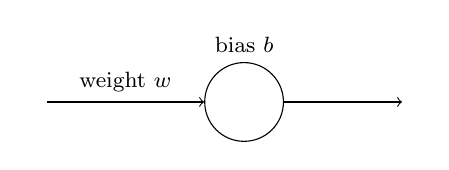
\begin{tikzpicture}[
    neuron/.style={circle,draw,inner sep=0pt,minimum size=10mm},
    font=\footnotesize
    ]

    \node (neuron) [neuron] {};
    \node (input) [left=2 of neuron] {};
    \node (output) [right=1.5 of neuron] {};

    \node [above] at (neuron.north) {bias $b$};

    \draw[->] (input) to node [above] {weight $w$} (neuron);
    \draw[->] (neuron) to (output);

  \end{tikzpicture}
\end{document}
